\section{Activity Diagrams Specification}
\label{appendix:activity-diagrams}
\subsection{Authentication Flow}

This activity diagram details the user authentication workflow in aBridgeAI. It shows how users log in through Google SSO, how the system verifies the local account and MFA requirement, creates an authenticated session, resolves roles and permissions, and handles logout.

\begin{figure}[H]
    \centering
    % Nhớ lưu ảnh tải về từ PlantUML thành tên act_auth.png
    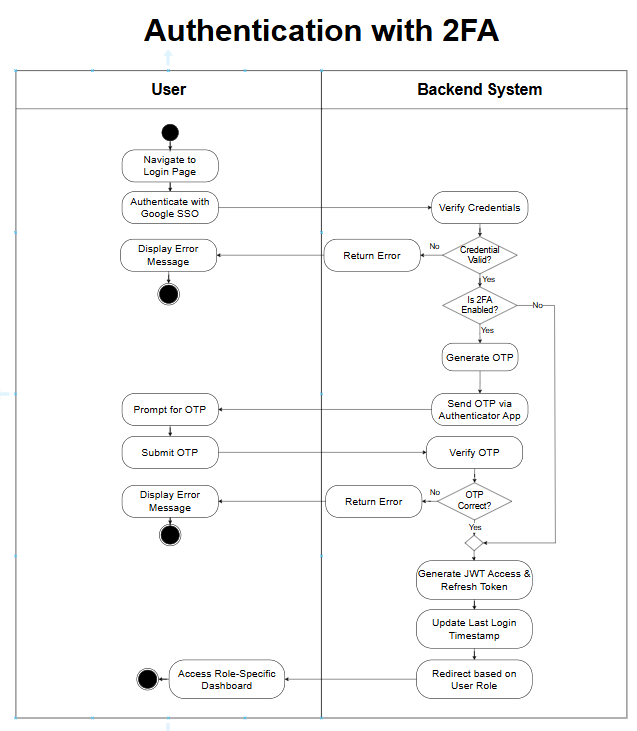
\includegraphics[width=0.85\textwidth]{graphics/act-diagrams/act_auth.png}   
    \caption{Activity Diagram: User Login with 2FA}
    \label{fig:act_auth}
\end{figure}

\subsection{Smart Content Ingestion Flow}

This activity diagram details the material ingestion workflow in aBridgeAI. It shows how teachers upload learning materials directly to object storage, how the backend verifies the upload and queues processing, and how the ingestion worker extracts, chunks, embeds, and stores content for retrieval.

\begin{figure}[H]
    \centering
    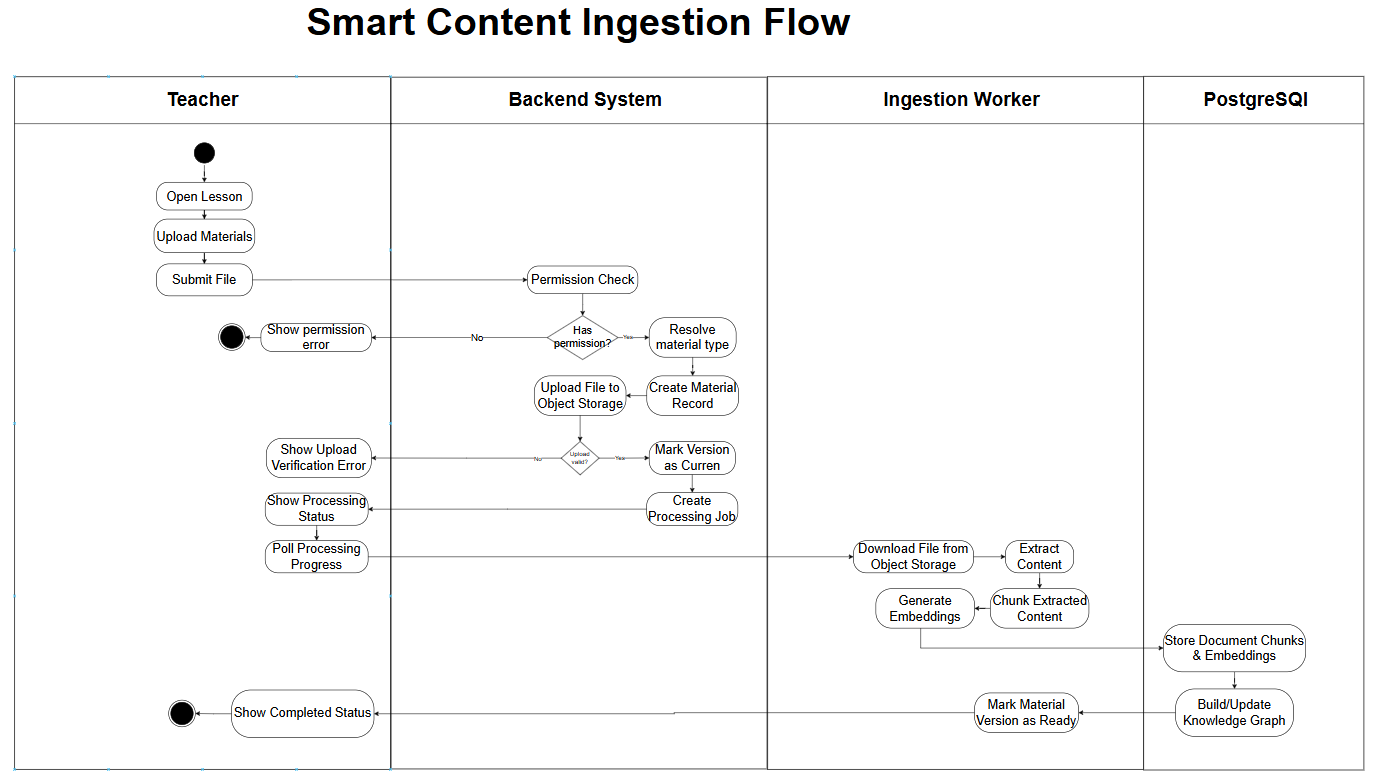
\includegraphics[width=0.95\textwidth]{graphics/act-diagrams/act_ingestion.png}
    \caption{Activity Diagram: Smart Content Ingestion and AI Parsing}
    \label{fig:act_ingestion}
\end{figure}

\subsection{Human-in-the-Loop Quiz Generation Flow}

This diagram maps the assessment creation lifecycle. It demonstrates the "Human-in-the-Loop" architecture where the teacher configures parameters, the AI generates a draft assessment based on the Knowledge Graph, and the teacher performs the final review and pedagogical adjustments before publishing the quiz to the students.

\begin{figure}[H]
    \centering
    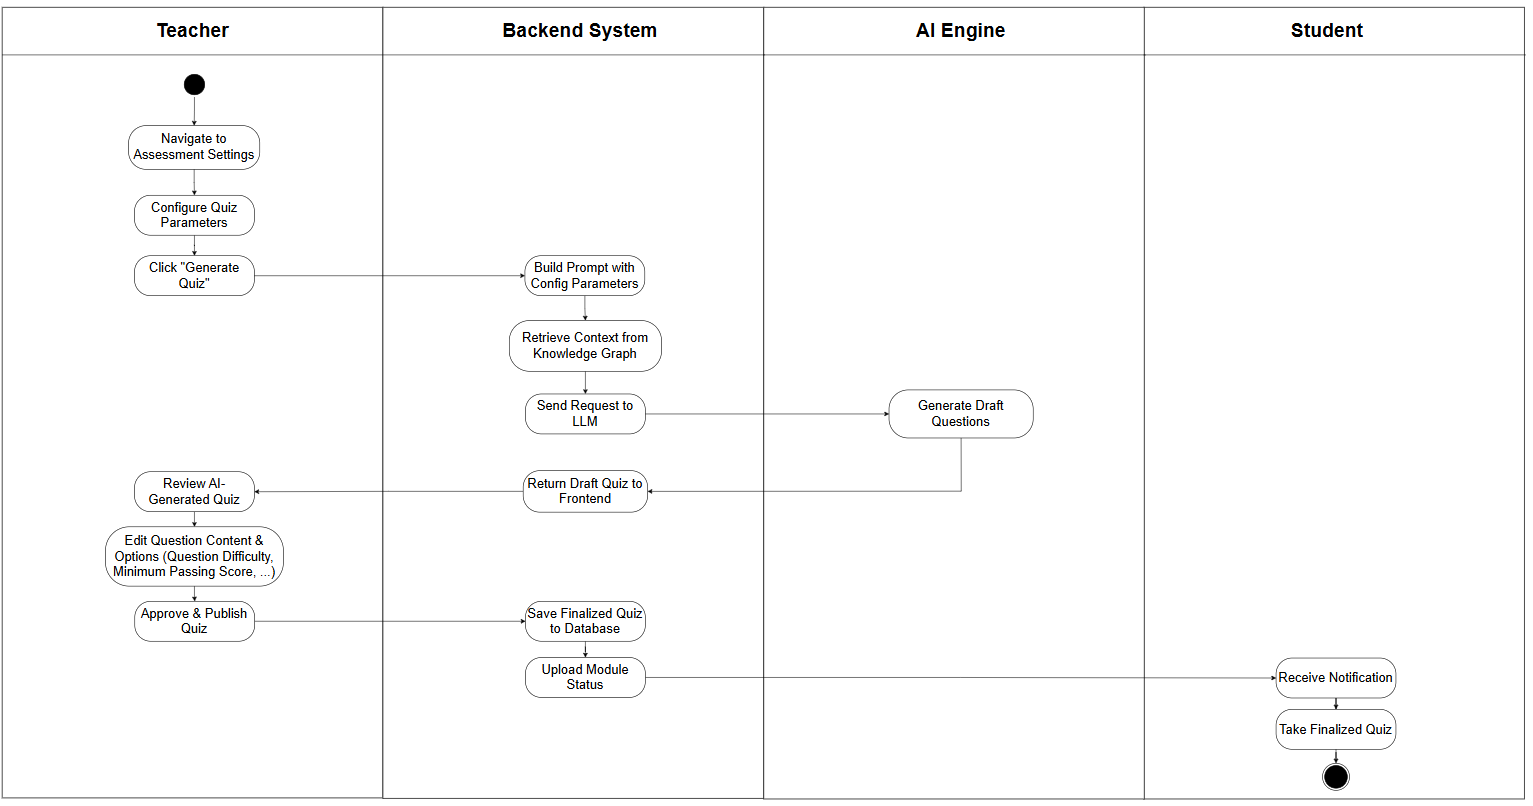
\includegraphics[width=1\textwidth]{graphics/act-diagrams/act_quiz_gen.png}
    \caption{Activity Diagram: HITL Quiz Generation and Execution}
    \label{fig:act_quiz_gen}
\end{figure}


\subsection{Native Mock Interview Flow}

The previous raster activity diagram described an older generic interview flow and has no editable source. It is replaced by the current native activity trace.

\begin{enumerate}
    \item Start or resume the persisted interview session; complete identity, audio, language, preparation, and readiness onboarding.
    \item Optionally connect a warm LiveKit room during onboarding; dispatch the native interviewer only after readiness and start the assessment clock.
    \item Receive either a final speech transcript or a typed \texttt{lk.chat} turn. For typed input, validate the action/key and persist a receipt before acknowledgement.
    \item Fold the answer into durable runtime state. Apply a fast provisional sufficiency probe, persist the state version, then server-select the next question or retain the current question within configured follow-up and hint bounds.
    \item Refresh the conversational state note. The LLM may phrase the next response and invoke guarded tools, while server policy remains authoritative for progression and completion.
    \item Publish TTS audio, transcription, and control snapshot; queue deferred reconciliation for richer analysis. On reconnect, republish a snapshot and re-read the current question.
    \item On model end or hard stop, close intake, drain bounded active work, flush transcript writes, submit once, enqueue terminal evaluation, and publish the final result when evaluation completes.
\end{enumerate}

This textual activity trace is aligned with Section~\ref{sec:impl_interviews}; it avoids presenting obsolete raster artwork as the deployed native architecture.

% \subsection{Bulk User Import and Validation Flow}

% This diagram maps the administrative workflow for bulk onboarding users via CSV files. It demonstrates the system's robust error-handling capabilities, illustrating how the validation engine processes the data, separates valid records from malformed ones, and dispatches asynchronous invitation emails.

% \begin{figure}[H]
%     \centering
%     % Nhớ lưu ảnh tải về từ PlantUML thành tên act_admin.png
%     \includegraphics[width=0.85\textwidth]{graphics/act_admin.png}
%     \caption{Activity Diagram: Bulk User Import via CSV}
%     \label{fig:act_admin}
% \end{figure}